\documentclass[a4paper, twoside]{article}

\usepackage[font={small,it}]{caption}
\usepackage{graphicx}
\usepackage{wrapfig}

\setlength{\oddsidemargin}{0in} \setlength{\evensidemargin}{0in}
\setlength{\textwidth}{6.2in}
\setlength{\topmargin}{-0.3in} \setlength{\textheight}{9.8in}

\title{CS25710 - Travel Trouble}
\author{Tom Leaman (thl5)}

\begin{document}
\maketitle
\newpage
%\tableofcontents
%\newpage

\section{Hardware}

\subsection{Components}

\subsubsection{Microcontroller}
\begin{wrapfigure}[9]{l}{0.25\textwidth}
	\vspace{-18pt}
	\begin{center}
		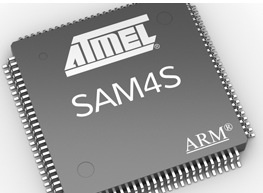
\includegraphics[scale=0.25]{images/atmel_sam4sd32.jpg}
	\end{center}
	\caption{Atmel SAM4SD32B}
\end{wrapfigure}

I began by looking at boards specifically designed for prototyping this kind of
device, such as the Arduino. These devices are typically very well supported,
often with a strong community of maker types. I decided against actually using
an Arduino, however, as it is slightly larger than the microcontroller specified
below and also requires more power.

In the end, I have specified an Atmel SAM4SD32B. This microcontroller can run at
a lower voltage (1.62 - 3.6v) and is small enough (I hope) to be attached to the
inside of even the smallest suitcase without too much hinderance to the case's
primary function of storing one's luggage!

The SAM4SD32B is equipped with 47 general I/O pins, an A/D converter, a
Synchronous Serial Controller and USB and SD connections. The microcontroller is
also capable of running in a number of low-power modes which will be a necessity
in keeping the device's power consumption to a minimum during its operational
life.

\subsubsection{Accelerometer/Gyro}
\begin{wrapfigure}{r}{0.25\textwidth}
	\begin{center}
		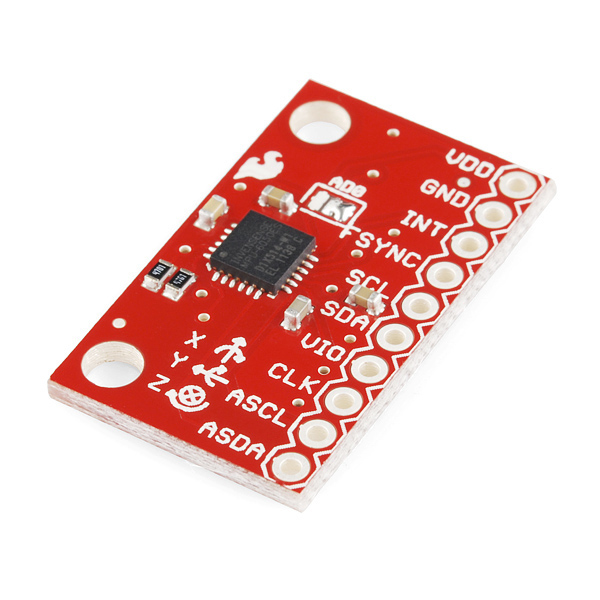
\includegraphics[scale=0.3]{images/mpu-6050.jpg}
	\end{center}
	\caption{InvenSense MPU-6050}
\end{wrapfigure}

I have selected a combined Accelerometer-Gyro, the MPU-6050. This is a 3-axis
Accelerometer and Gyro built into a single board. The device is capable of
measuring movement within a range of programmatically selected ranges which may
allow the client to record a range of movement events during the device's
deployment.

I intend to make use of the accelerometer's available interrupt routines to
wake-up the microcontroller when movement is occurring. I am intending to
collect data approximately every 0.5 seconds during 'gentle' movement (such as
might occur when walking around with the case). I intend to capture data far
more rapidly during 'shock' events, I believe capturing around 1000 times per
second (for half a second or so) should be adequate.

I did consider using a seperate accelerometer and gyro but these typically will
not only take more physical space and power but also, many of the 3-axis gyros I
found were actually more expensive on their own than the combined IMU specified
above.

\subsubsection{GPS}
\begin{wrapfigure}{l}{0.25\textwidth}
	\vspace{-35pt}
	\begin{center}
		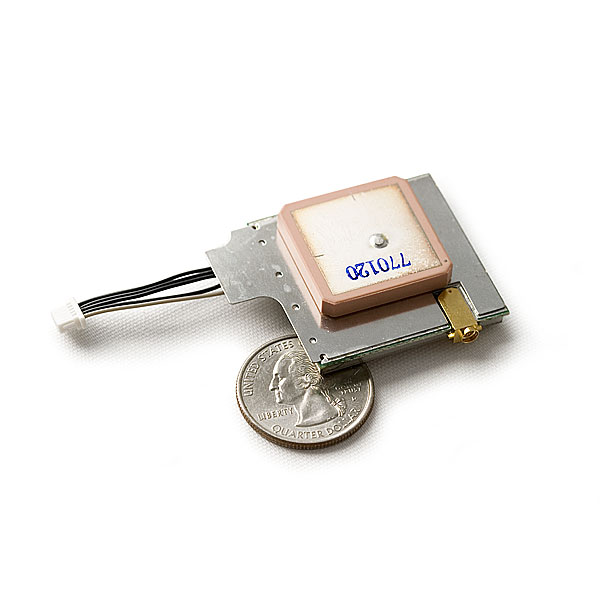
\includegraphics[scale=0.2]{images/em-408.jpg}
	\end{center}
	\vspace{-20pt}
	\caption{GlobalSat EM-408}
\end{wrapfigure}

When selecting a GPS, I tried to find one with a good signal strength (it will
likely be subject to a few layers of various materials which may hamper its
ability to communicate with the necessary satellites. I also tried to find
devices with an on-board antenna as this will reduce the overall form factor.

In the end, I have specified the EM-408. This is capable of 10m accuracy (which
I anticipate will be more than enough for this application), and a high degree of
sensitivity (-159dBm). The EM-408 is capable of outputting data in a number of
well supported formats and more consultation would be required with the client
to acertain exactly what data they require for their analysis.

\clearpage
\subsubsection{Temperature}
\begin{wrapfigure}{r}{0.25\textwidth}
	\vspace{-40pt}
	\begin{center}
		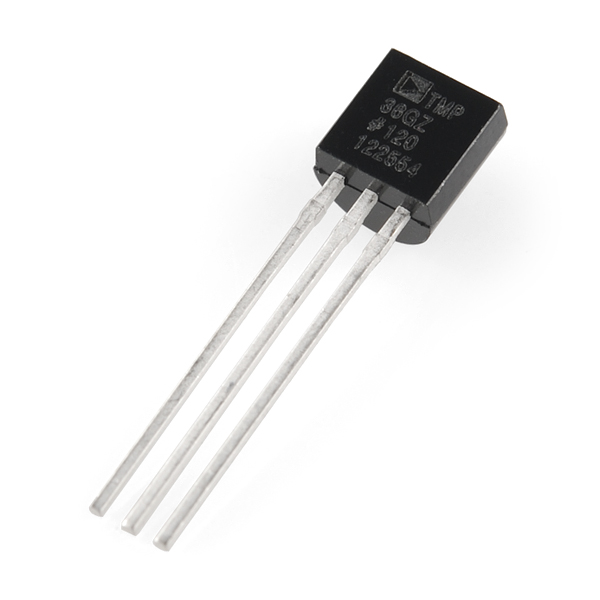
\includegraphics[scale=0.4]{images/tmp36.jpg}
	\end{center}
	\caption{Analog Devices TMP36}
\end{wrapfigure}

I have specified the use of a TMP36 temperature sensor. This is a very small,
low-powered component which can measure temperature accurate to within 1 or 2
degrees (accuracy is reduced at higher temperatures).

\subsubsection{Cells}
\begin{wrapfigure}{l}{0.25\textwidth}
	\vspace{-20pt}
	\begin{center}
		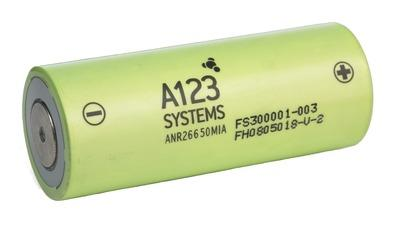
\includegraphics[scale=0.15]{images/a123.jpg}
	\end{center}
	\caption{OSN Power Tech A123}
	\vspace{-20pt}
\end{wrapfigure}

I have calculated the the device will draw around 130mA when capturing data and
around 0.2mA in standby mode. I am assuming the device will be in capture mode
for approx 5\% of its operation. This works out at 2247.84mAh during the
device's two-week operation.

I have decided to specify a Lithium Ion battery. This has a very low rate of
self discharge and should provide a reasonable stable power supply during
operation. These cells also have the added benefit of being rechargable and
should last for around 2000 uses if cared for properly.

I have decided to specify the use of 1 A123 (ANR26650M1B) cell. This cell will output
3.3v at up to 150A (capacity 2500mAh. Unfortunately, I have only been able to
locate 1 supplier for this exact model of cell which requires a minimum order of
50 pieces. I would be keen to discuss alternative power configurations with the
client, but I believe this cell to be the most ideal for the task at hand.

\subsection{Major alternatives}
Aside from using an Arduino as the base for the project (outlined above),
another option would be to use a smartphone with an open, extensible software
platform inlcuded (for example, and Android phone). These devices typically have
many of the sensory devices required to achieve the necessary functionality
(with the omission, perhaps, of temperature sensing). I believe this would
significantly reduce the overall cost and development time.

I believe the main drawback of this approach is that the device would not be as
flexible in terms of component selection (it would be a much larger operation
to, for example, install a different GPS sensor) and the components it contains
may not be able to sense accurately or fast enough to capture the level of data
required to be useful to the client.

\subsection{Data storage}
I intend to make use of an SD card to hold the data captured by the device.
These are very compact and reasonably priced storage media and will allow the
client to simply transfer the card into their own machine to interpret and
analyse the data. In addition to this, the microcontroller has 2MB of flash
memory built-in which I intend to use as a write cache before the data gets sent
to the SD card. This should avoid a bottle-neck of data trying to be written to
disk during shock events.

In addition to the accelerometer and gyro information being captured (outlined
above), I intend to capture GPS and temperature data around once every 5mins while the device is
moving.

\clearpage
\subsection{Connection diagram}
\begin{center}
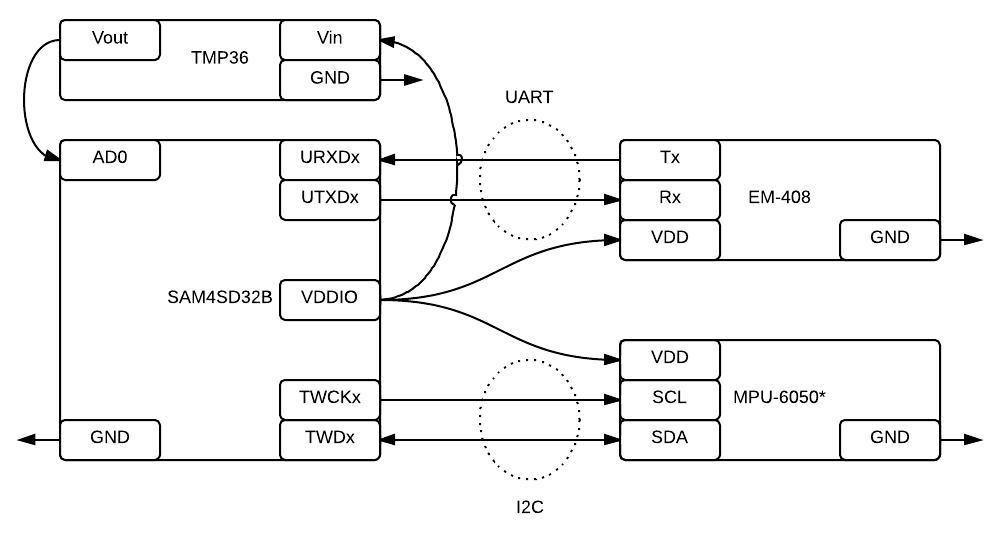
\includegraphics[scale=0.45]{images/connectiondiagram.jpg}
\end{center}
* I believe the MPU-6050 will also require the VLOGIC and INT pins to be
connected to the microcontroller to enable the microcontroller to wake from
sleep mode when movement commences. I have not been able to acertain from the
datasheets available where these connections should be made, however. I believe
that the connections are available on the microcontroller though and someone
with more experience than myself should not have a problem locating the correct
connections.

\subsection{Power consumption}

\begin{tabular}{|l|l|l|}
	\hline
	\textbf{Device} & \textbf{Active state} & \textbf{Idle state} \\
	\hline
	\hline
	SAM4SD32B & 80mA & 32$\mu$A \\
	MPU-6050 & 4.1mA & 115$\mu$A \\
	EM-408 & 44mA & N/A \\
	TMP36 & 50$\mu$A & 0.5$\mu$A \\
	\hline
	\hline
	Total & 128.15mA & 147.5$\mu$A \\
	\hline
\end{tabular}

\subsection{Dimensions}

\subsection{Bill of materials}

\section{Software}

\subsection{Block diagram}

\subsection{Detail} % TODO think of a less shit name

\subsection{Development plan}

\subsection{Usage procedure}

\section{References}
\begin{itemize}
	\item{Microcontroller - Atmel SAM4SD32B - http://www.atmel.com/devices/SAM4SD32B.aspx}
	\item{IMU - InvenSense MPU-6050 - https://www.sparkfun.com/products/11028}
	\item{GPS - GlobalSat EM-408 - https://www.sparkfun.com/products/8234}
	\item{Temperature - Analog Devices TMP36 - https://www.sparkfun.com/products/10988}
	\item{Cell - OSN Power Tech A123 -
		http://www.alibaba.com/product-gs/742803918/LiFePO4\_battery\_A123\_26650\_with\_2500mAh.html}
\end{itemize}

\end{document}

